\documentclass[12pt]{article}
\usepackage{latexsym}
\usepackage{epsfig}
\usepackage{amsmath}
\usepackage[edges]{forest}


\setlength{\topmargin}{0in}
\setlength{\leftmargin}{0in}
\setlength{\textwidth}{6in}
\setlength{\textheight}{9.5in}
\setlength{\parindent}{0.2in}
\setlength{\parskip}{.08in}
\voffset = -.45in
\hoffset = -.5in
\def\filledbox{\vrule height 1.8ex width .8ex depth -.1ex } % square bullet
\newcommand{\qed}{\large ~$\Box$ \normalsize}
%
%\newtheorem{thm}{Theorem}
%\newenvironment{theorem}{\begin{thm}\ \rm}{\end{thm}}
%
%\newtheorem{lem}{Lemma}
%\newenvironment{lemma}{\begin{lem}\ \rm}{\end{lem}}
%
\newtheorem{theorem}{Theorem}
\newtheorem{lemma}{Lemma}
\newtheorem{corollary}{Corollary}
\newenvironment{proof}{{\noindent \bf Proof\ \ }}{\qed}
\newenvironment{proofsketch}{{\noindent {\bf Proof}\ (sketch)\ \ }}{\qed}
%
\def\shh{\skew3\hat{\hat s}}
\def\dhh{\skew6\hat{\hat d}}
\begin{document}
\newcommand{\I}{\mbox{{\em Int}}}
\newcommand{\lt}{\mbox{{\em left}}}
\newcommand{\rt}{\mbox{{\em right}}}
\newcommand{\ld}{\Delta^l}
\newcommand{\rd}{\Delta^r}
\newcommand{\lsp}[1]{\large\renewcommand{\baselinestretch}{#1}\normalsize}
\newcommand{\hsp}{\hspace{.2in}}

\def\Endwhile{\mbox{\bf endwhile\ }}
\def\Or{\mbox{\bf or\ }}
\def\Do{\mbox{\bf do\ }}
\def\Downto{\mbox{\bf downto\ }}
\def\Int{\mbox{\bf int\ }}
\def\To{\mbox{\bf to\ }}
\def\Repeat{\mbox{\bf repeat\ }}
\def\Until{\mbox{\bf until\ }}
\def\Return{\mbox{\bf return\ }}
\def\Not{\mbox{\bf not\ }}
\def\And{\mbox{\bf and\ }}
\def\For{\mbox{\bf for\ }}
\def\Foreach{\mbox{\bf foreach\ }}
\def\Else{\mbox{\bf else\ }}
\def\Elseif{\mbox{\bf elseif\ }}
\def\End{\mbox{\bf end\ }}
\def\If{\mbox{\bf if\ }}
\def\Mod{\mbox{\bf \ mod\ }}
\def\Then{\mbox{\bf then\ }}
\def\While{\mbox{\bf while\ }}
\def\Output{\mbox{\bf output\ }}


\lsp{1}
\pagestyle{plain}
\hfill Ally Smith
\begin{center}
{\bf
% Worksheet title here %
Dynamic Programming Project
}
\end{center}

\begin{description}
    \item [Recursive Implementation]\ 
    
    Below is the code I used for my recursive implementation of the algorithm.
    When run with the parameters $p = 3,~t = 16$ the function is called 753,665 times.
    \begin{center}
        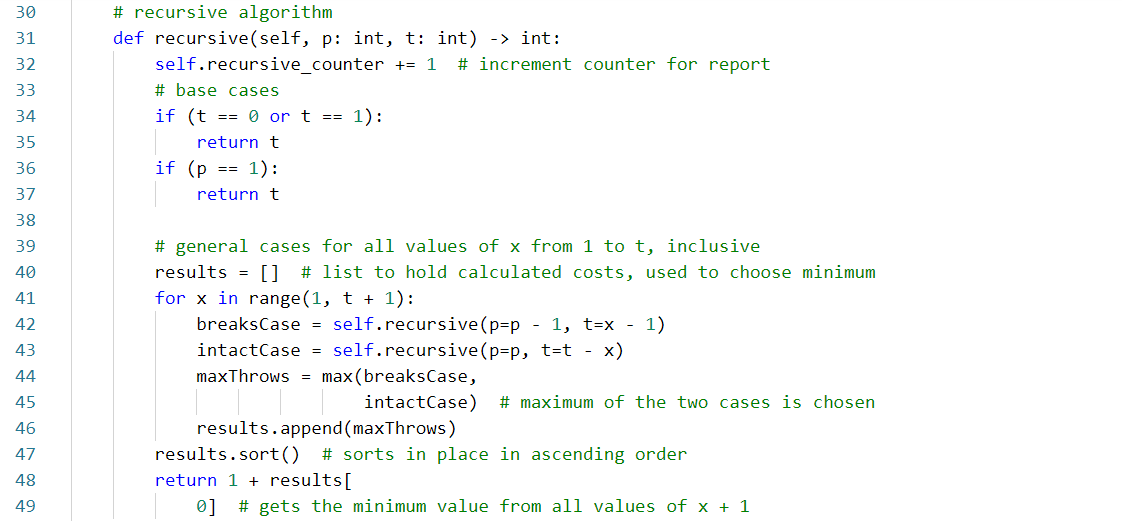
\includegraphics[width=5.5in]{recursive.png}
    \end{center}

    \item [Recursive Runtime Analysis] (measured in ms)
    
    \begin{center}
        \begin{tabular}{|c|c|c|c|c|c|}\hline
            $\frac{t}{p}$ & 10 & 12 & 15 & 18 & 20 \\\hline
            2 & 1 & 2 & 20 & 170 & 716 \\\hline
            4 & 7 & 39 & 499 & 5,942 & 29,772\\\hline
            8 & 13 & 117 & 2,958 & 65,222 & \\\hline
            12 & 13 & 134 & 3,398 & & \\\hline
        \end{tabular}
    \end{center}
    As can be seen in the table above, the runtime increases greatly with slight
    changes in $t$. Additionally, higher values of $p$ begin to affect the runtime
    more as $t$ increases. For example, the runtime of $p = 8,~t = 10$ is fairly
    close to that of $p = 4,~t = 10$, but $p = 8,~t = 15$ is far greater than
    $p = 4,~t = 15$.

    \pagebreak
    \item [Dynamic Programming Implementation]\ 
    
    Below is the code I used for my dynamic programming implementation of the algorithm.
    \begin{center}
        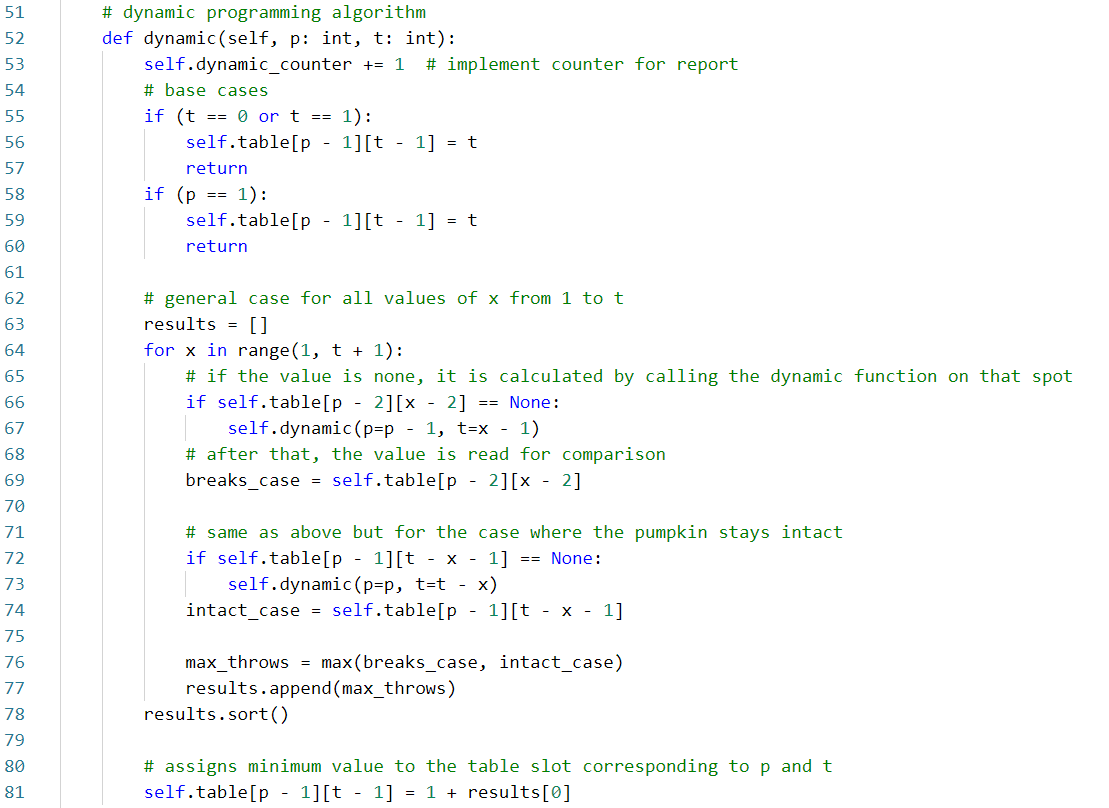
\includegraphics[width=5.5in]{dynamic.png}
    \end{center}

    \item [Dynamic Runtime Analysis] (measured in ms)
    
    \begin{center}
        \begin{tabular}{|c|c|c|c|c|c|c|c|c|c|c|}\hline
            $\frac{t}{p}$ & 20 & 40 & 60 & 80 & 100 & 120 & 140 & 160 & 180 & 200 \\\hline
            20 & 1 & 6 & 14 & 26 & 41 & 64 & 86 & 114 & 141 & 176 \\\hline
            40 & 1 & 7 & 20 & 39 & 70 & 107 & 148 & 202 & 256 & 328 \\\hline
            80 & 1 & 7 & 20 & 47 & 89 & 143 & 217 & 308 & 411 & 538 \\\hline
            120 & 1 & 7 & 21 & 47 & 91 & 153 & 239 & 353 & 481 & 634 \\\hline
            160 & 1 & 7 & 21 & 48 & 91 & 153 & 239 & 359 & 517 & 695 \\\hline
        \end{tabular}
    \end{center}
    As can be seen in the above table, growth in $t$ leads to an increased runtime
    with $p$ held constant. Similarly, an increase $p$ can lead to an increased
    runtime, however this value seems to max out as $p \to t$. If $p$ and $t$ are
    increasing simultaneously, then the runtime will increase dramatically.
\end{description}

\end{document} 
